%%%%%%%%%%%%%%%%%%%%%%%%%%%%%%%%%%%%%%%%%%%%%%%%%%%%%%%%%%%%%%%%%%%%%%%%%%%%%%%%
%2345678901234567890123456789012345678901234567890123456789012345678901234567890
%        1         2         3         4         5         6         7         8
\documentclass[letterpaper, 10 pt, conference]{ieeeconf}  % Comment this line out
                                                          % if you need a4paper
%\documentclass[a4paper, 10pt, conference]{ieeeconf}      % Use this line for a4

\usepackage{float}
                                                          % paper
% uso paquete bookmark para tener bien los outlines.
\usepackage{bookmark}

% Configuro el idioma.
\usepackage[utf8]{inputenc} % Importante para mantener acentos.
\usepackage[spanish, activeacute]{babel} % Requiere: texlive-lang-spanish. Por primera vez hay que ejecutar: texconfig init> log

% Paquete para poder usar acentos en $$.
\usepackage{mathtools}
%\setmathfont{XITS math}

% Para los diagramas de flujo
\usepackage{tikz}
\usetikzlibrary{shapes.geometric, arrows}

% Elementos del diagrama
\tikzstyle{startstop} = [rectangle, rounded corners, 
minimum width=6em, 
minimum height=2em,
text centered, 
draw=black, 
fill=red!30]

\tikzstyle{io} = [trapezium, 
trapezium stretches=true, % A later addition
trapezium left angle=70, 
trapezium right angle=110, 
minimum width=6em, 
minimum height=2em, text centered, 
draw=black, fill=blue!30]

\tikzstyle{block} = [rectangle, 
minimum width=8em, 
minimum height=3em, 
text centered, 
text width=7.5em, 
draw=black, 
fill=white!30]

\tikzstyle{def} = [rectangle, 
minimum width=14em, 
minimum height=3em, 
text centered, 
text width=12em, 
draw=black, 
fill=purple!30]

\tikzstyle{swap_proccess} = [rectangle, 
minimum width=8em, 
minimum height=2em, 
text centered, 
text width=8em, 
draw=black, 
fill=orange!30]

\tikzstyle{process} = [rectangle, 
minimum width=6em, 
minimum height=2em, 
text centered, 
text width=6em, 
draw=black, 
fill=orange!30]

\tikzstyle{decision} = [diamond, 
minimum width=6em, 
minimum height=6em, 
text centered, 
draw=black, 
fill=green!30]
\tikzstyle{arrow} = [thick,->,>=stealth]

\usepackage{siunitx}

% package to get \url
\usepackage{hyperref}
\hypersetup{
  colorlinks=true,
  linkcolor=magenta,
  filecolor=magenta,
  citecolor=magenta,      
  urlcolor=magenta,
}

% Graficos electrónicos
\usepackage[RPvoltages]{circuitikz}

\IEEEoverridecommandlockouts                              % This command is only
                                                          % needed if you want to
                                                          % use the \thanks command
\overrideIEEEmargins
% See the \addtolength command later in the file to balance the column lengths
% on the last page of the document

\usepackage{graphicx}
\usepackage{graphics}

% styling for matlab/octave code.
\usepackage{matlab-prettifier}
% Configuracion, con esto puede agregar ñ.
\lstset{
  literate={ñ}{{\~n}}1
}

\usepackage{listings}

% The following packages can be found on http:\\www.ctan.org
%\usepackage{graphics} % for pdf, bitmapped graphics files
%\usepackage{epsfig} % for postscript graphics files
%\usepackage{mathptmx} % assumes new font selection scheme installed
%\usepackage{times} % assumes new font selection scheme installed
\usepackage{amsmath} % assumes amsmath package installed
%\usepackage{amssymb}  % assumes amsmath package installed

\title{\LARGE \bf Amplificador de audio con boostrapping}

\author{
  Tom\'as Vidal\\
  {\it Circuitos Electróicos II}\\
  {\it Facultad de Ingenier\'ia, UNLP, La Plata, Argentina.}\\
  {\it 30 de Septiembre, 2024.}
}                                            % <-this % stops a space

\begin{document}
\maketitle
\thispagestyle{empty}
\pagestyle{empty}

\section{Placa}
\begin{figure}[H]
  \centering
  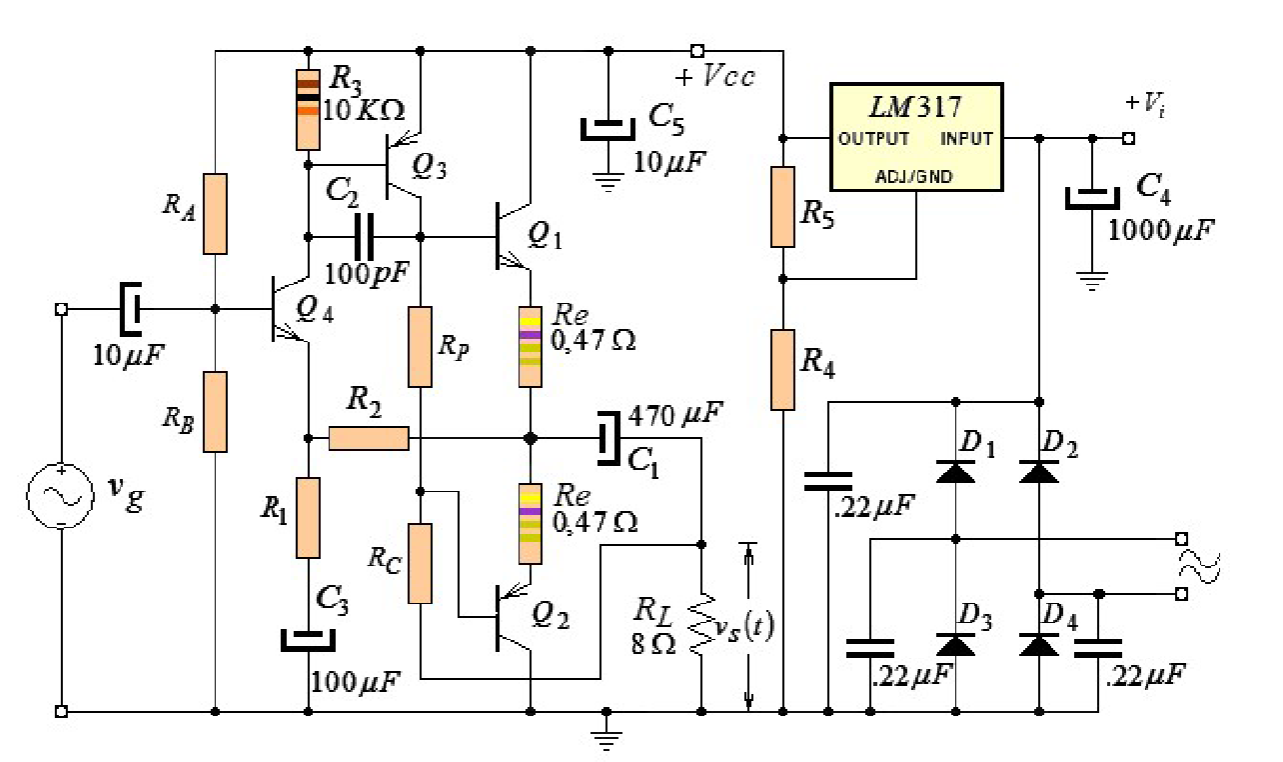
\includegraphics[width=0.43\textwidth]{./imagenes/placa.png}
  \caption{Esquemático de la placa a desarrollar}
  \label{fig:placa}
\end{figure}
El circuito a implementar consiste de una \textbf{fuente de alimentación}, un \textbf{par complementario} que amplifica la corriente, y dos etapas de \textbf{emisor común} realimentadas que amplifican tensión. Además hay una rama de realimentación de \textbf{boostrapping}.

\section{Cálculo de los parámetros de diseño}
\subsection{Fuente de alimentación}
\begin{figure}[H]
  \centering
  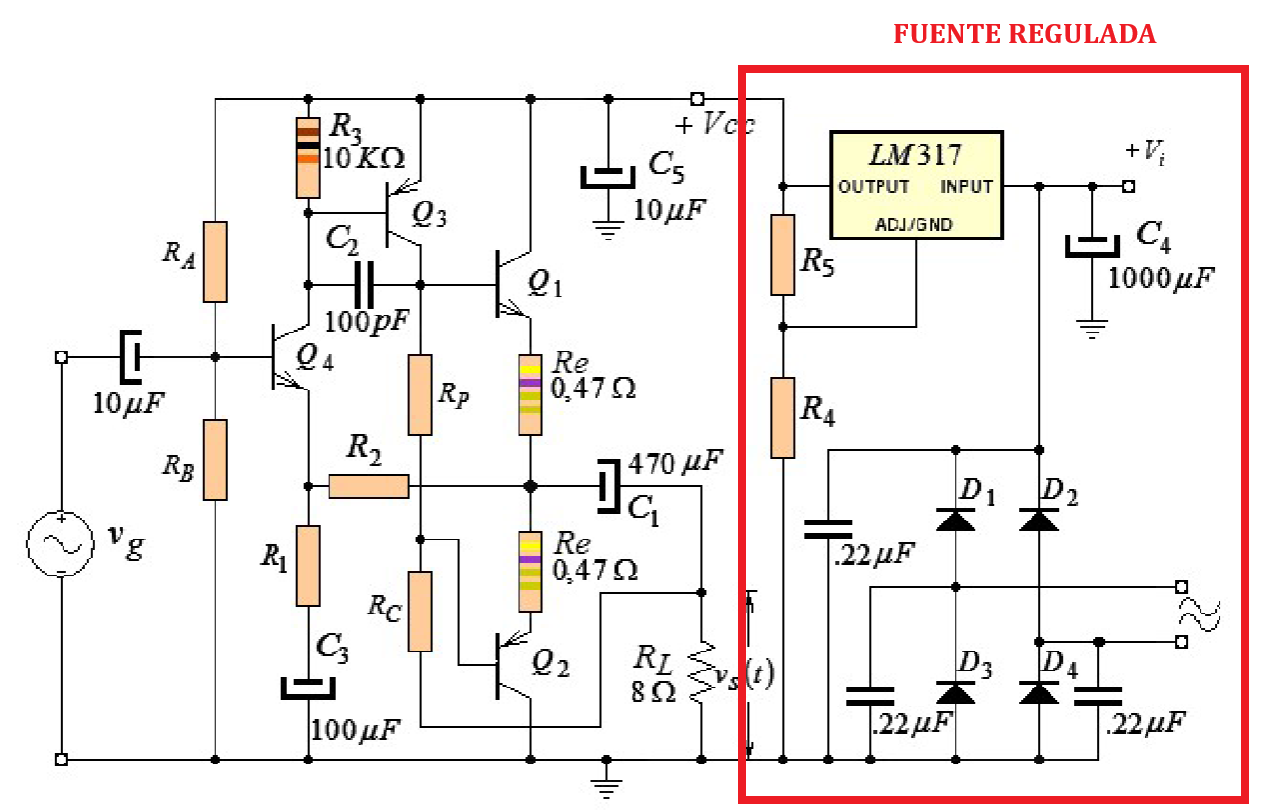
\includegraphics[width=0.43\textwidth]{./imagenes/placa_fuente.png}
  \caption{Sección de la fuente regulada}
  \label{fig:placa_fuente}
\end{figure}

Especificaciones de entrada:
\begin{itemize}
  \item{$220V_{ef} AC$ a $50Hz$ con un ripple del $10\%$}
\end{itemize}
Requerimientos de salida:
\begin{itemize}
  \item{13V con ripple máximo de $8\%$}
\end{itemize}

Para cumplir con estas condiciones se empleó un análisis con las siguientes consideraciones:
\begin{itemize}
  \item{60V y 1.5A máximos en el LM317}
  \item{3V mínimos entre entrada y salida del LM317}
  \item{La corriente de ajuste del LM317 tiene que ser del orden de los $\qty{}{\micro\ampere}$, contra la de $R_1$ y $R_2$ que debe ser del orden de los $mA$}
\end{itemize}

Partiendo de que en la salida del regulador se tiene una carga de \qty{50}{\ohm}, y se quiere una tensión \textit{estable} de \qty{13}{\volt}; se puede calcular la corriente máxima en la carga, para lo cual se consideró que la carga puede variar un $20\%$ (como medida de seguidad, ya que menor carga será mayor corriente), es decir, puede variar a \qty{40}{\ohm} en el peor caso, resultando así en una corriente máxima de \qty{325}{\milli\ampere}. \\
Sabiendo la tensión mínima del regulador, y agregandole un márgen de seguridad de \qty{2}{\volt} (es decir un $66\%$); se calcula la resistencia equivalente del LM317: 
\begin{equation} \label{eq:lm317_resistance}
  R_{LM317} = \frac{5V}{325mA} \cong \qty{15}{\ohm}
\end{equation}
\textit{El margen del $66\%$ es elevado ya que se involucran muchos efectos que pueden hacer variar la tensión, y la consecuencia de ajustar a un valor más alto no es tan ponderante, ya que se trabaja con poca potencia.} \\

Por lo que se puede calcular la tensión máxima requerida en el secundario con las curvas de \textbf{Schade}; haciendo la carga del rectificador filtrado \qty{65}{\ohm} (la carga original de \qty{50}{\ohm} en serie con los \qty{15}{\ohm}), como se muestra en la figura \ref{fig:lm317_como_resistencia}
\begin{figure}[H]
  \centering
  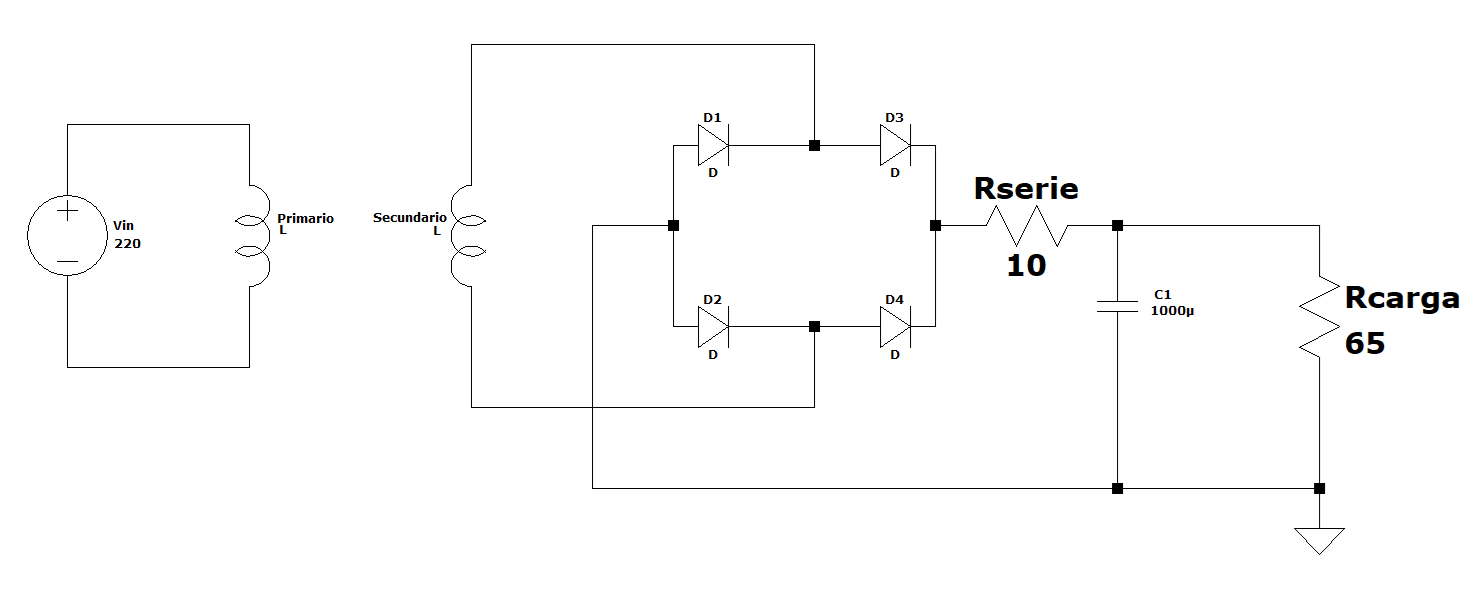
\includegraphics[width=0.43\textwidth]{./imagenes/circ_eq_lm137_carga.png}
  \caption{Circuito equivalente con LM317 como resistencia}
  \label{fig:lm317_como_resistencia}
\end{figure}

% TODO: preguntar por qué el ripple calculado con Schade no se corresponde en la simulación.
Tomando $\frac{R_s}{R_{carga}}\% = \frac{10}{65}*100 \cong 15\%$ ($R_s$ es un dato conocido); y calculando $wR_{carga}C \cong 20$, se puede obtener de las curvas de \textbf{Schade} el ripple en el capacitor, que será aproximadamente de $3\%$, y la tensión máxima del secundario, que será de $26V$ pico para el peor caso, es decir cuando en el primario se tenga $90\%$ de la tensión. Con estos datos se puede obtener la relación de espiras entre el primario y el secundario del transformador:
\begin{equation}
  \frac{V_1}{V_2} = \frac{N_1}{N_2} = N \cong 10.78
\end{equation}

\begin{figure}[H]
  \centering
  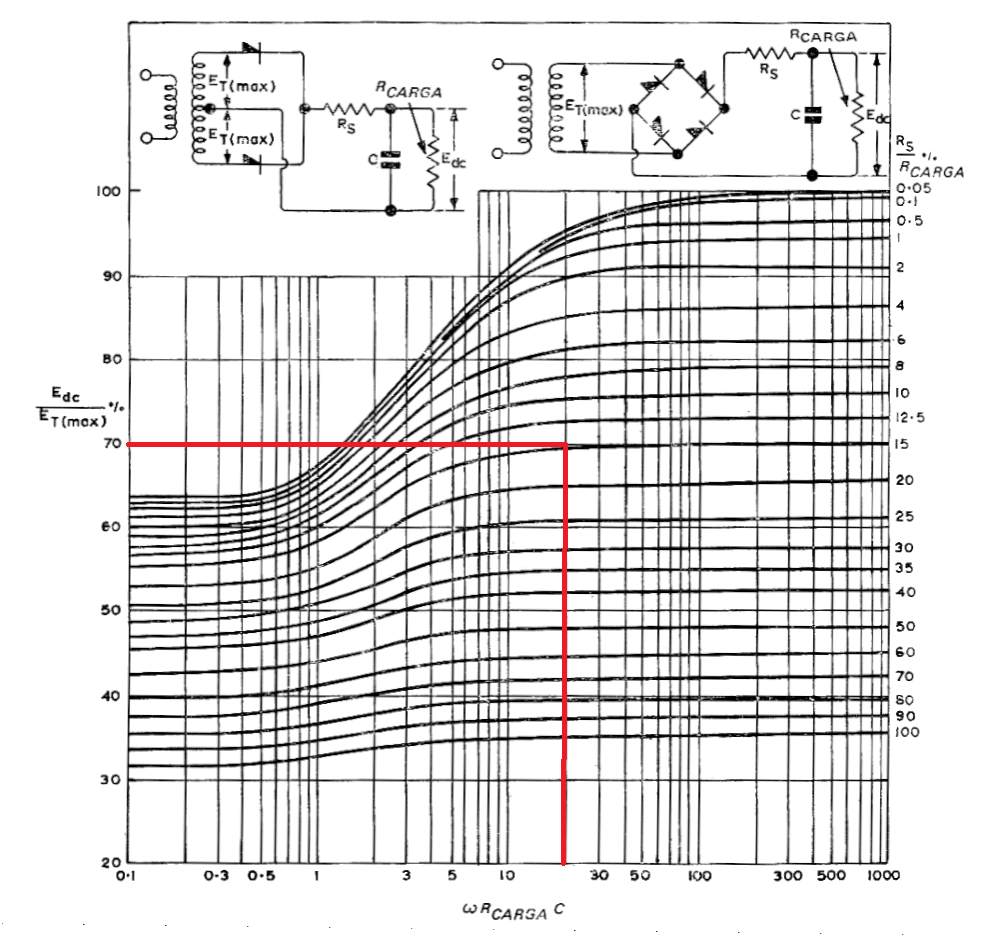
\includegraphics[width=0.43\textwidth]{./imagenes/schade_edc_et.png}
  \caption{Curva de Schade}
  \label{fig:schade_edc_sobre_etmax}
\end{figure}

\textit{Los cálculos anteriores se consideraron para el caso de carga nominal y carga mínima, que es el peor caso, cuando más corriente se demanda en la carga. $N \cong 10.78$ es el caso pesimista.}

\subsection{Amplificador de tensión realimentado}
\begin{figure}[H]
  \centering
  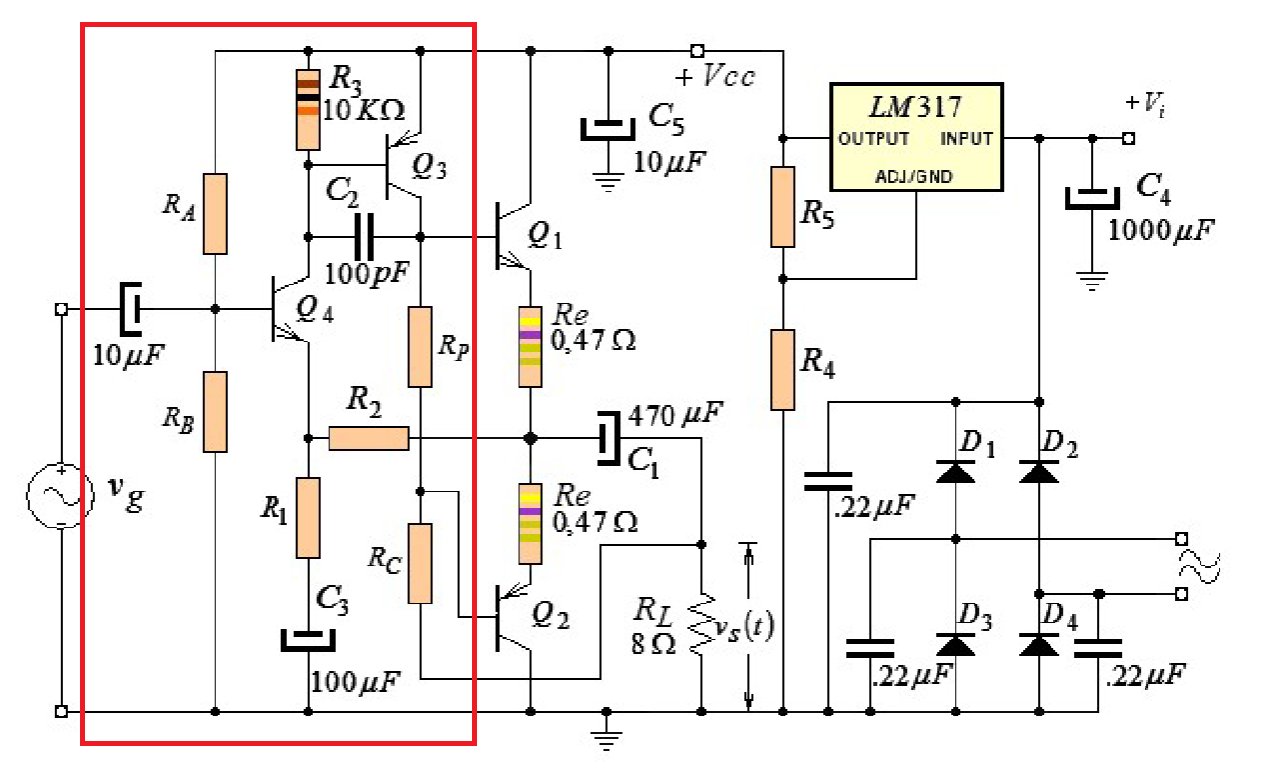
\includegraphics[width=0.43\textwidth]{./imagenes/placa_ampli_realimentado.png}
  \caption{Sección de amplificación de tensión realimentada}
  \label{fig:ampl_tension_reali}
\end{figure}
Los transistores $Q_3$ y $Q_4$, en configuración \textbf{emisor común}, en combinación con el divisior resistivo $R_1$ y $R_2$; forman un \textbf{amplificador de tensión realimentado negativamente}. El propósito del mismo es tener una ganacia en tensión elevada, proporcionada por $Q_3$ y $Q_4$, y la realimentación estabiliza la tensión a coste de ganancia. Estos componentes se pueden pensar como el siguiente circuito equivalente (fig \ref{fig:circ_eq_ampli_reali}), tanto se cumpla que la gananacia de tensión proporsionada por $Q_3$ y $Q_4$ sea lo \textit{suficientemente}\footnote{Es decir que se cumpla $a\beta \gg 1$. Se puede asumir que lo hace, ya que las etapas de emisior común se ajustan para que así lo sea.} elevada.

\begin{figure}[H]
  \centering
  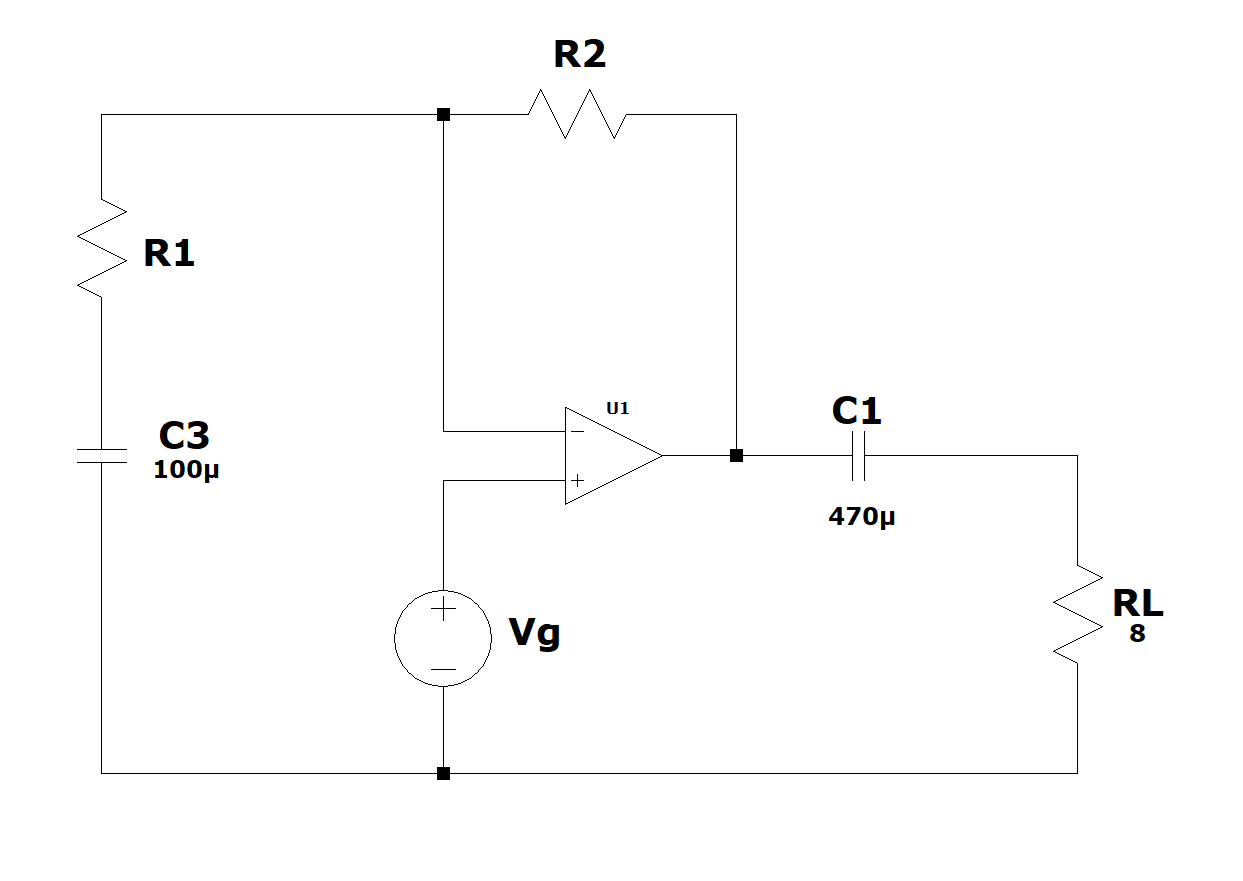
\includegraphics[width=0.43\textwidth]{./imagenes/circ_eq_ampli_real.png}
  \caption{Circuito equivalente del amplificador realimentado}
  \label{fig:circ_eq_ampli_reali}
\end{figure}

La ganacia de este circuito equivalente \textit{(en frecuencias medias)} se puede ajustar fácilmente con $R_1$ y $R_2$, sabiendo:
\begin{equation} \label{eq:ganancia_ampli_real}
  G_0 = 1 + \frac{R_2}{R_1}
\end{equation}

Además en la red de realimentación aparece el polo de baja frecuencia generado por $C_1$ y $R_2 + R_L$; que se hizo dominante sobre el polo generado por $R_1$ y $C_3$, resultando en que $(R_2+R_L) > R_1$




\end{document}